\chapter{Features e Controlli}
\section{Spiegazione}
Tutti le GUI presentano una ricerca per Titolo/Nome. Inoltre la GUI "Catalogo Libri" presenta una ulteriore ricerca per Cognome dell'autore. In generale vengono implementate diverse JComboBox per il filtraggio di attributi all'interno dell tuple.

\begin{figure}[hbt]
\subsection{StartPage}
La gui di partenza apre a diverse opzioni: \begin{itemize}
	\item Acceder al catalogo
	\item Andare al link della documentazione che rimanda a github
	\item Andare al link delle pagine degli autori
\end{itemize}
\begin{center}
	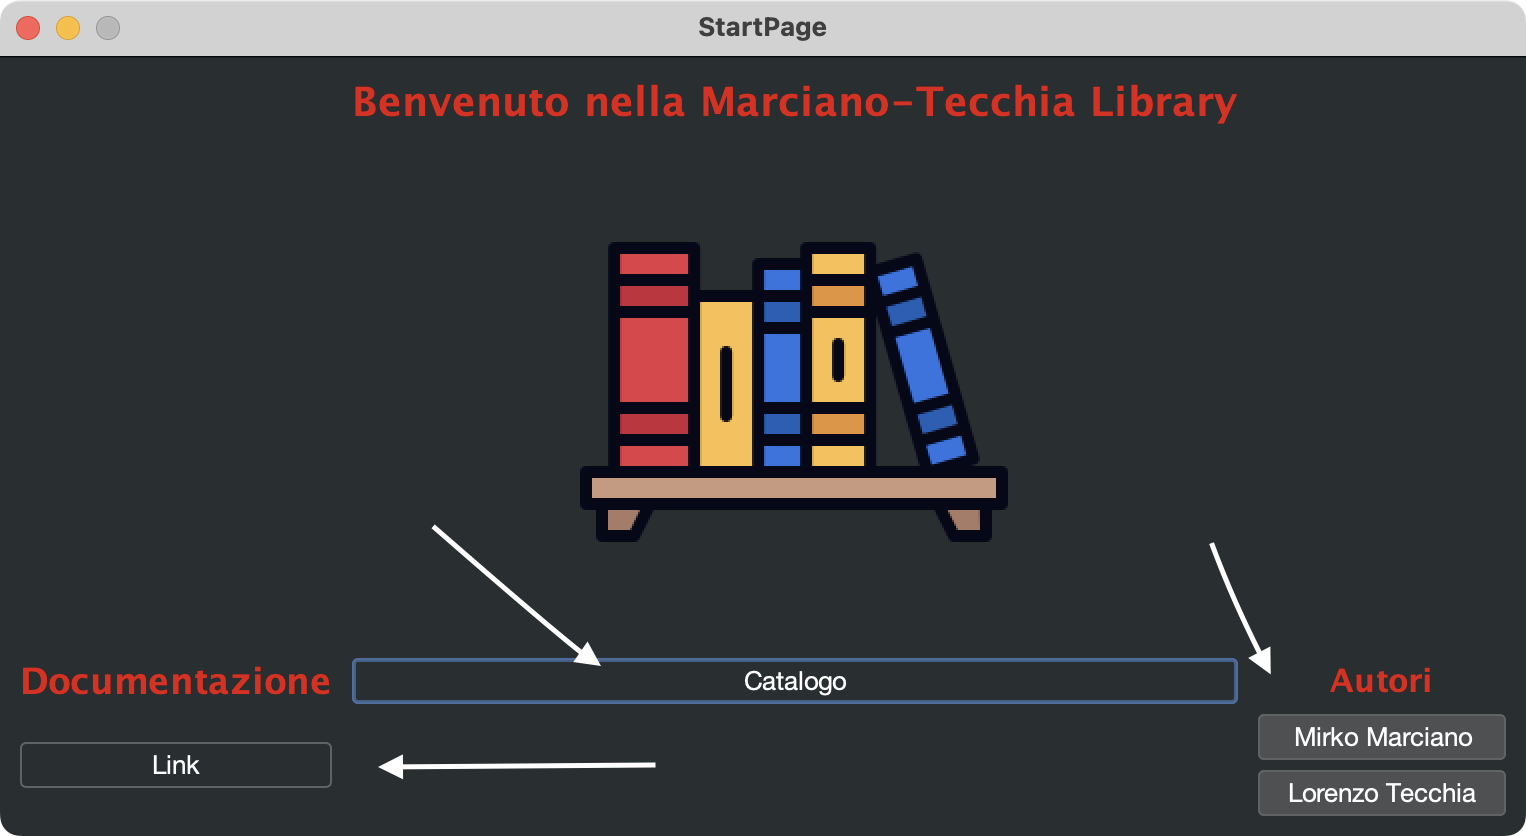
\includegraphics[width=\textwidth]{Immagini/startpageScreen.png}
  \caption{StartPageGUI}
\end{center}
  
\end{figure}

\begin{figure}[hbt]
\subsection{Catalogo Libri}
E' stato preso come esempio la GUI "Catalogo Libri", la quale presenta il maggior numero di funzionalità. Come mostrato nella figura sottostante la ricerca per cognome dell'autore riporta alla sola tupla di libri il cui autore corrisponde a quello cercato all'interno della GUI.
\begin{center}
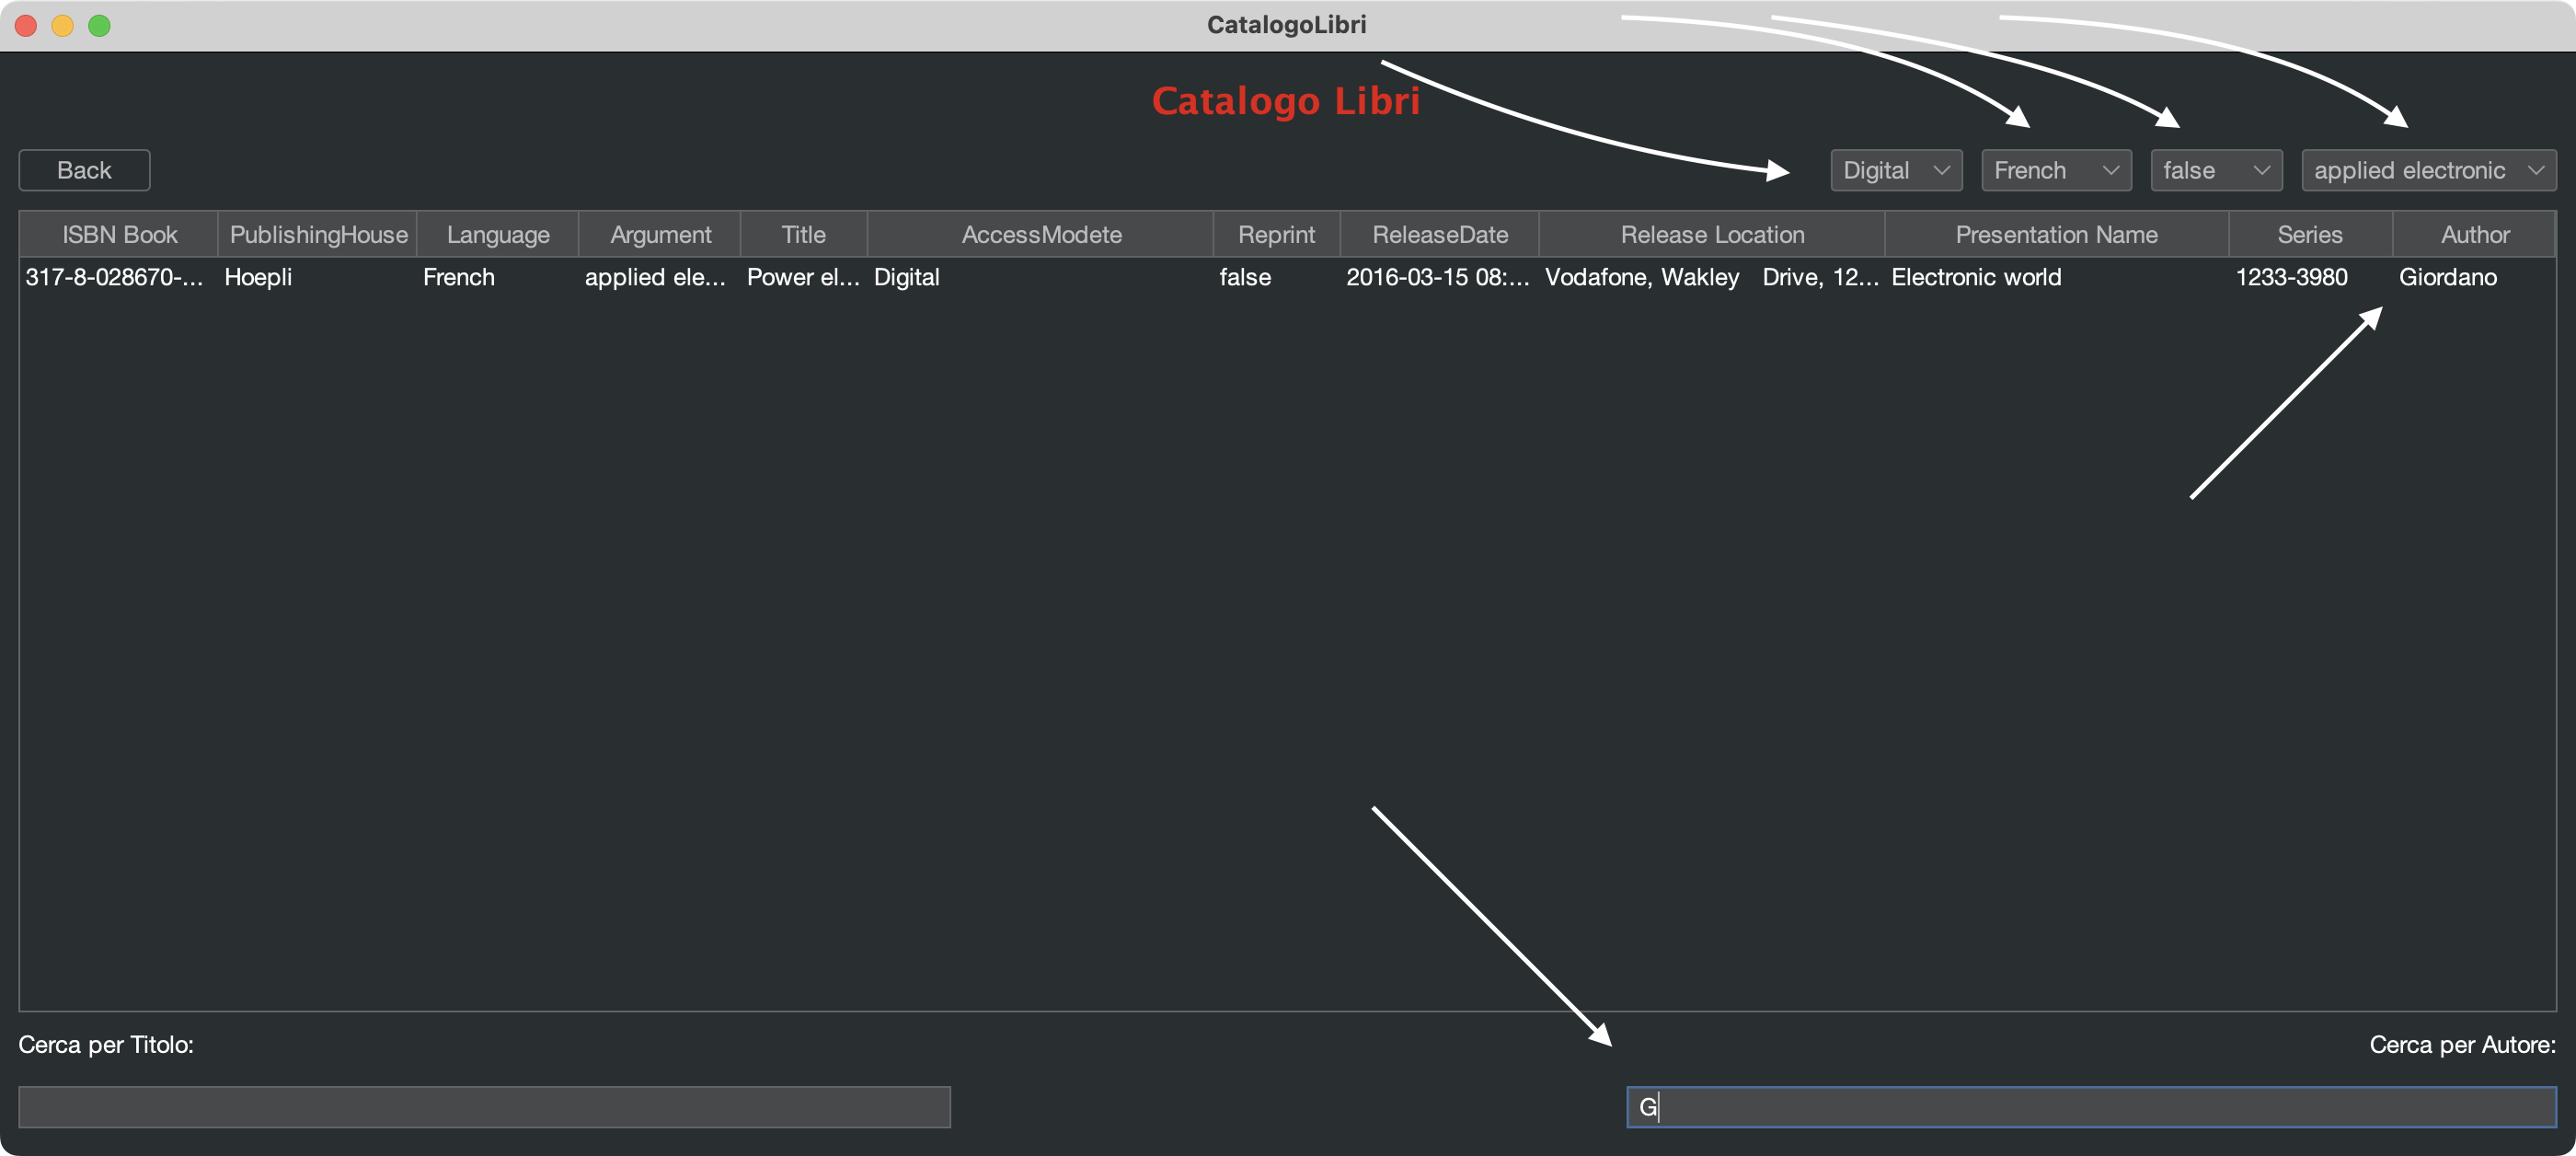
\includegraphics[width=\textwidth]{Immagini/catalogolibriScreen.png}
  \caption{CatalogoLibriGUI}
	
\end{center}
  \end{figure}

\begin{figure}[hbt]
\subsection{Catalogo Collane}
Come ultimo esempio è stato presa la GUI "CatalogoCollane" per mostrare la funzionalità di una qualsiasi JComboBox assieme alla ricerca per titolo, basta appunto inserire una sola lettera, anche all'interno della parola stessa, per ricevere le opzioni corrispondenti.
\begin{center}
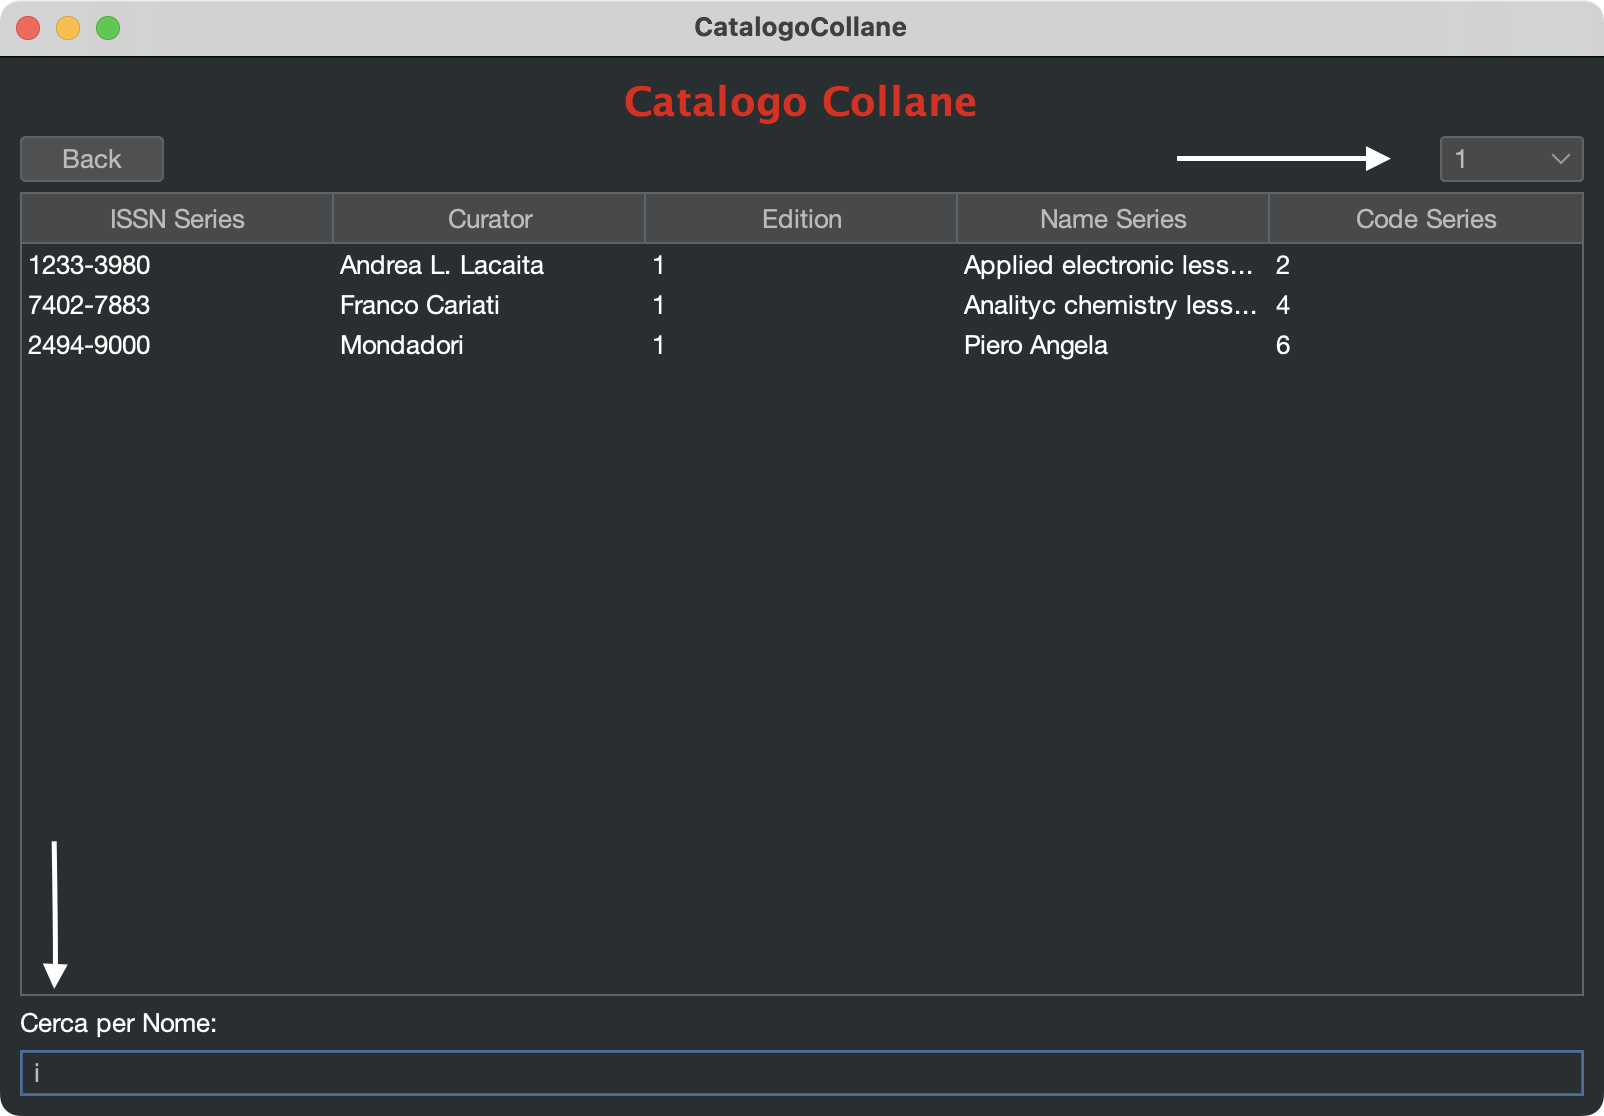
\includegraphics[width=\textwidth]{/Users/lorenzotecchia/Documents/ESAMI/ProgettoOOBD/ProgettoOOBD_LaTeX_Object/Immagini/catalogocollaneScreen.png}
  \caption{CatalogoCollaneGUI}	
\end{center}
  
\end{figure}

